\documentclass[a4paper,12pt]{article}

% 页面设置
\usepackage[top=2.54cm, bottom=2.54cm, left=1.91cm, right=1.91cm]{geometry}

% 中文支持
\usepackage[UTF8]{ctex}
\usepackage{fontspec}

% 数学公式支持
\usepackage{amsmath}
\usepackage{amssymb}
\usepackage{amsfonts}
\usepackage{amsthm}

\usepackage{enumitem}

% 定理环境定义
\newtheorem*{pf}{Proof}
\newtheorem*{sol}{Solution}

% 图形支持
\usepackage{graphicx}
\usepackage{tikz}

% 超链接支持
\usepackage{hyperref}
\hypersetup{
    colorlinks=true,
    linkcolor=blue,
    filecolor=magenta,
    urlcolor=cyan,
}

% 行距设置
\linespread{1.25}

% 标题信息
\title{CourseName HomeworkName}
\author{袁子强\hspace{1cm} 2025533009}
% \date{}

\begin{document}

\maketitle

\begin{enumerate}
      \item[7.] 确定并画出以下函数的定义域，并指出它们是否是区域，是否是闭区域.
            \begin{enumerate}[label=(\protect\the\numexpr2*\arabic*\relax)]
                  \item $z = \sqrt{x - 2y^2}$;
                        \begin{sol}
                              由定义域条件得 $x - 2y^2 \geq 0$，即 $x \geq 2y^2$。

                              该区域包含边界，因此是闭区域；但不是开集，故不是区域。

                              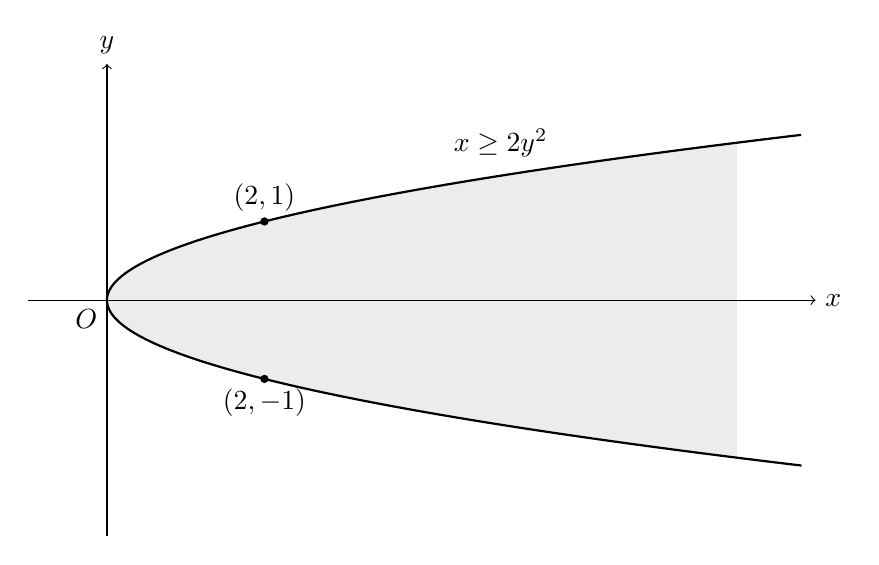
\begin{tikzpicture}[scale=1]
                                    % 填充区域 x ≥ 2y²（浅灰色阴影）
                                    \fill[gray!30, opacity=0.5, domain=-2:2, samples=200]
                                    plot (\x*\x*2, \x) -- (8,2) -- (8,-2) -- cycle;

                                    % 绘制直角坐标系
                                    \draw[->] (-1, 0) -- (9, 0) node[right] {$x$};
                                    \draw[->] (0, -3) -- (0, 3) node[above] {$y$};
                                    \draw (0,0) node[below left] {$O$};

                                    % 绘制边界抛物线 x=2y²（实线，因包含等号）
                                    \draw[thick, black, domain=-2.1:2.1, samples=200]
                                    plot (\x*\x*2, \x);

                                    % 标注关键点
                                    \fill (2,1) circle (1.5pt);
                                    \fill (2,-1) circle (1.5pt);
                                    \node at (2,1.3) {$(2,1)$};
                                    \node at (2,-1.3) {$(2,-1)$};

                                    % 标注区域方程
                                    \node at (5, 2) {$x \geq 2y^2$};
                              \end{tikzpicture}
                        \end{sol}
                  \item $z = \sqrt{\sin(x^2 + y^2)}$;
                        \begin{sol}
                              由定义域条件得 $\sin(x^2 + y^2) \geq 0$。

                              由于 $x^2 + y^2 \geq 0$，因此 $x^2 + y^2 \in [2k\pi, (2k+1)\pi]$，其中整数 $k \geq 0$。

                              上述多个区间互不连通，因此定义域既不是区域，也不是闭区域。

                              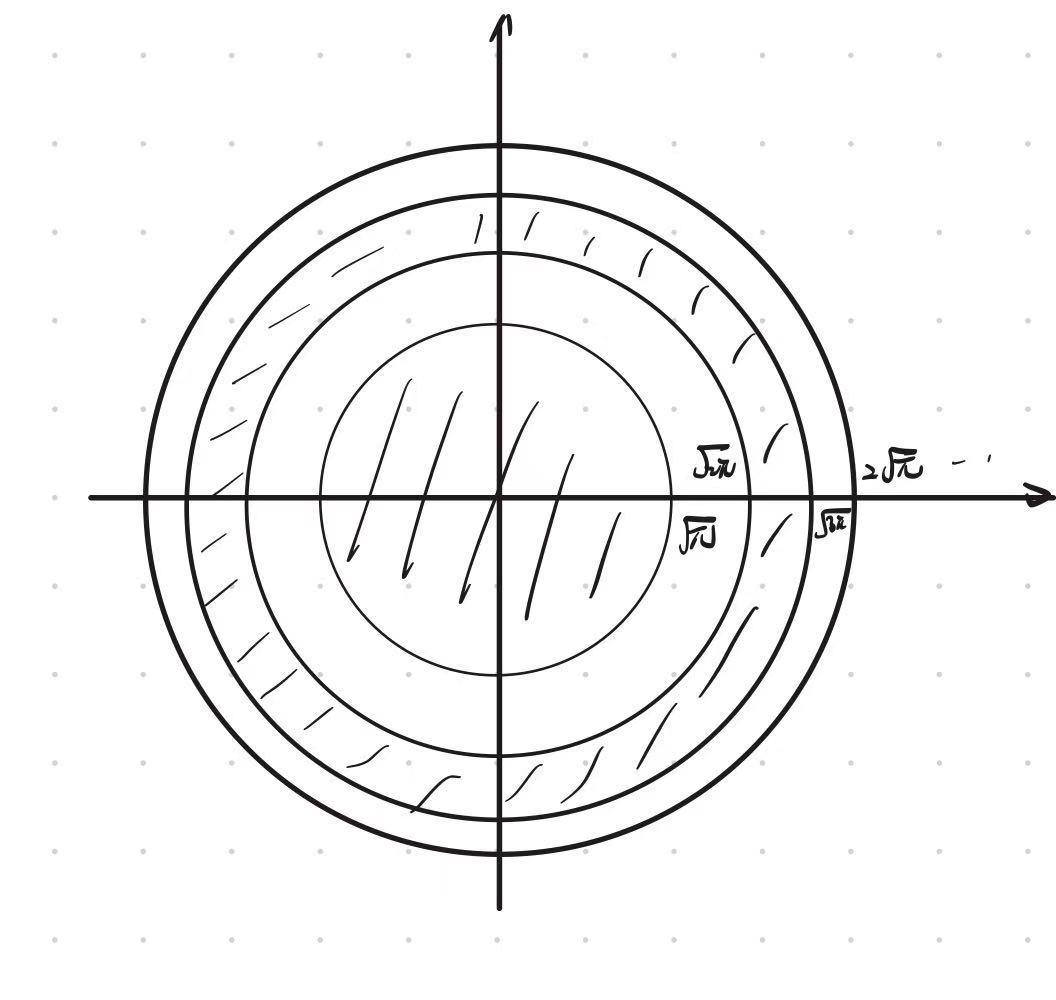
\includegraphics[height=4cm]{2-1-1}
                        \end{sol}
                  \item $z = \sqrt{\cos x \sin y}$;
                        \begin{sol}
                              由定义域条件得 $\cos x \sin y \geq 0$，即 $\cos x \geq 0,\,\sin y \geq 0$ 或 $\cos x \leq 0,\,\sin y \leq 0$。

                              因此定义域为
                              $$
                                    \begin{cases}
                                          x \in \left[\left(2k-\frac{1}{2}\right)\pi, \left(2k+\frac{1}{2}\right)\pi\right] \\
                                          y \in [2k\pi, 2(k+1)\pi]
                                    \end{cases}
                                    \quad\text{或}\quad
                                    \begin{cases}
                                          x \in \left[\left(2k+\frac{1}{2}\right)\pi, \left(2k+\frac{3}{2}\right)\pi\right] \\
                                          y \in [(2k-1)\pi, 2k\pi]
                                    \end{cases}
                              $$
                              其中 $k$ 为整数。

                              上述多个区域互不连通，因此定义域既不是区域，也不是闭区域。

                              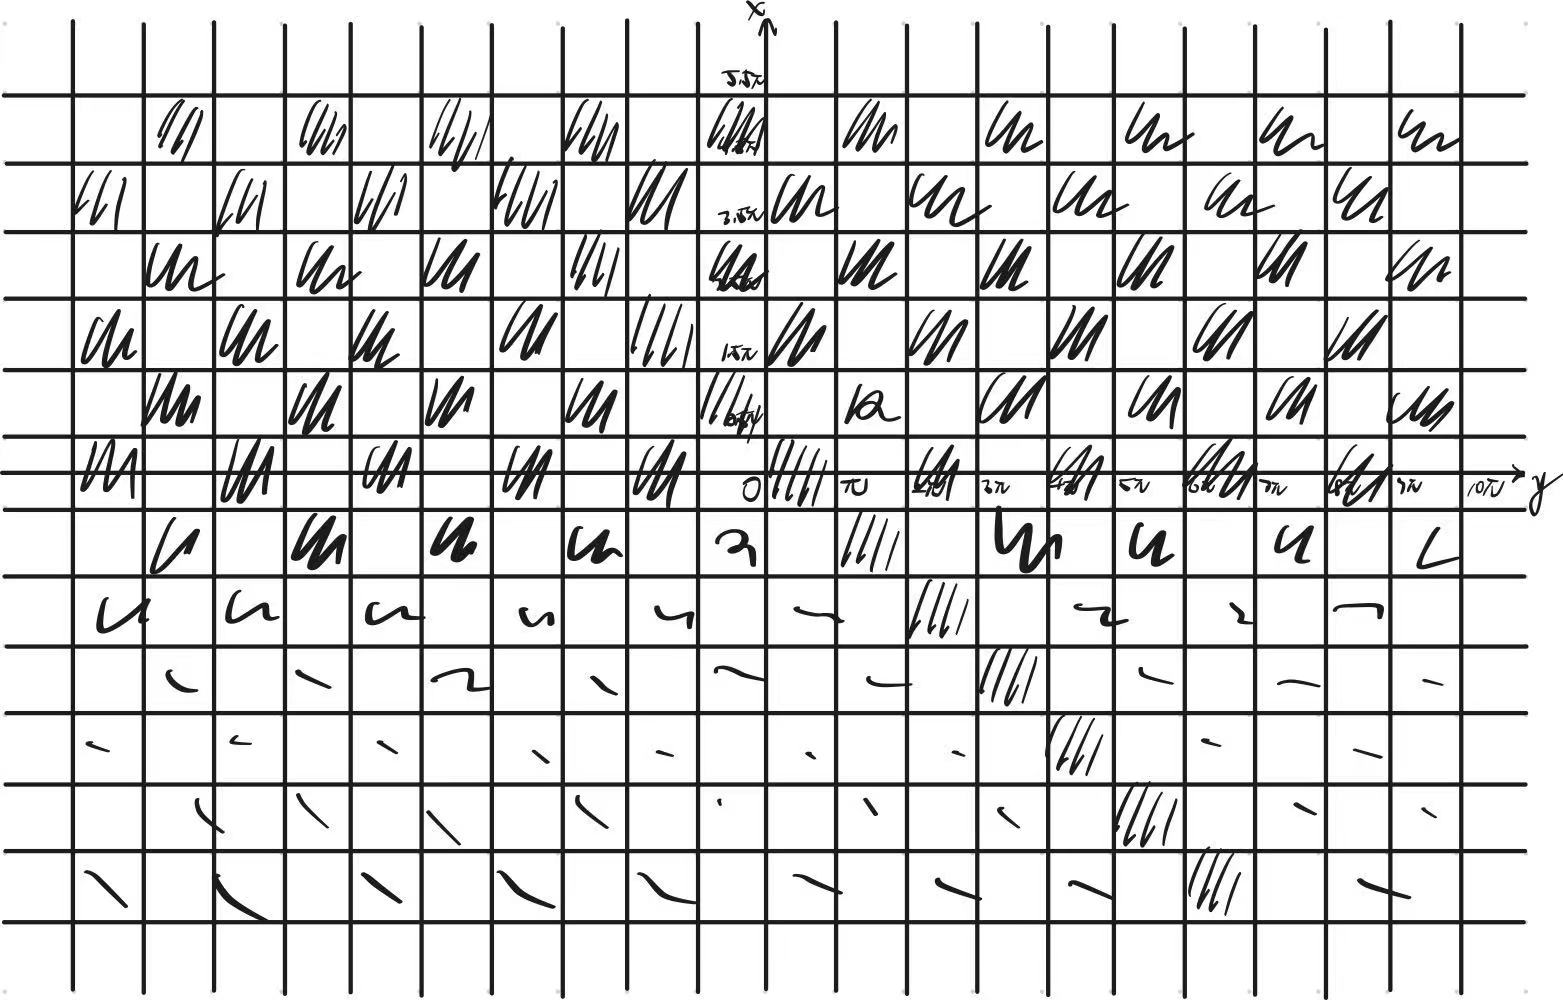
\includegraphics[height=4cm]{2-1-2}
                        \end{sol}
                  \item $u = \sqrt{2az - x^2 - y^2 - z^2}\ (a > 0)$.
                        \begin{sol}
                              由定义域条件得 $2az - x^2 - y^2 - z^2 \geq 0$。

                              整理得 $x^2 + y^2 + z^2 - 2az + a^2 \leq a^2$，即 $x^2 + y^2 + (z-a)^2 \leq a^2$。

                              该区域表示以 $(0, 0, a)$ 为球心、$a$ 为半径的球体（包含边界），因此是闭区域；但不是开集，故不是区域。

                              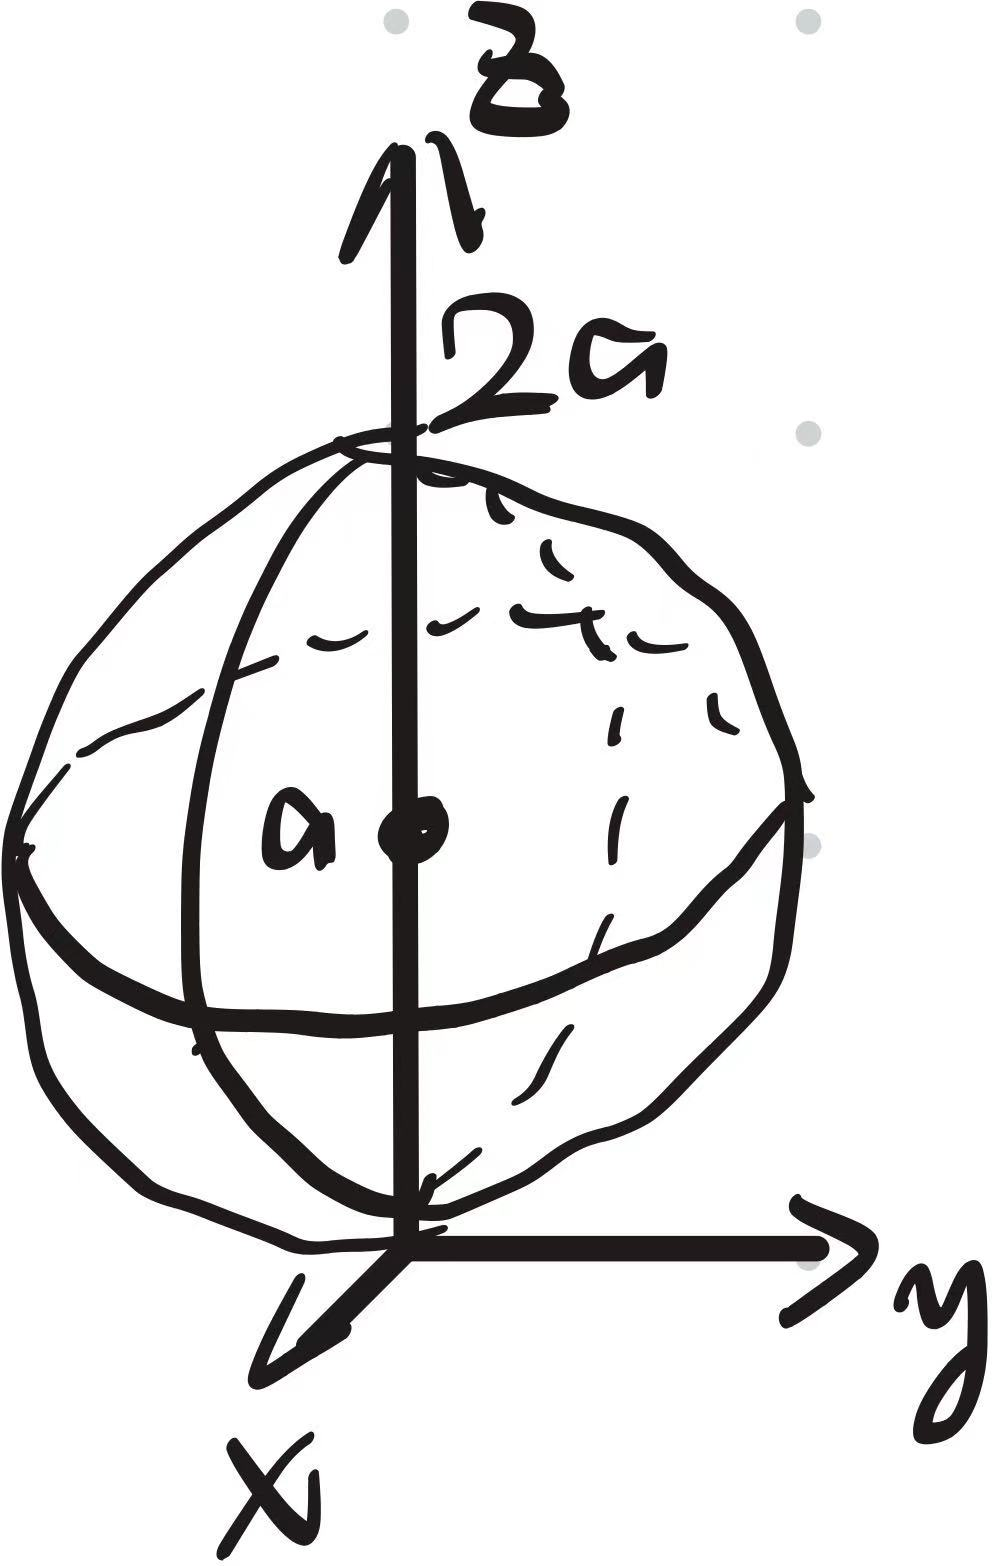
\includegraphics[height=4cm]{2-1-3}
                        \end{sol}
            \end{enumerate}

      \item[9.] 一个变量的一般形式的 $n$ 次多项式共有 $n+1$ 项单项式 $x^0,x^1,\dots,x^n$，如果对于两个变量而言，单项式定义为 $x^k y^l$，次数定义为 $k+l$，问一般形式的 $n$ 次二元多项式一共有多少项，推广到 $k$ 个变量的情形呢？
            \begin{sol}
                  设次数为 $n$，变量数为 $k$，则每项的形式为 $t_1^{l_1} t_2^{l_2} \dots t_k^{l_k}$，其中 $l_i \geq 0$ 且 $l_1 + l_2 + \dots + l_k = n$。因此，问题等价于将 $n$ 次分配给 $k$ 个变量，每个变量的次数可以为 $0$。

                  采用隔板法：考虑在 $n+k$ 个位置中放置隔板，使得每个变量至少分配到 $1$ 次，再减去多余的部分。具体而言，需要在 $n+k-1$ 个空隙中插入 $k-1$ 个隔板，故总项数为
                  $$
                        \binom{n+k-1}{k-1} = \frac{(n+k-1)!}{n!(k-1)!}.
                  $$
            \end{sol}

      \item[12.] 设 $f\left(x+y,\frac{y}{x}\right) = x^2 - y^2\ (x \neq 0)$，求 $f(2,3), f(x,y)$.
            \begin{sol}
                  令 $u = x + y$，$v = \frac{y}{x}$，解得 $x = \frac{u}{v+1}$，$y = \frac{uv}{v+1}$。

                  代入原式得
                  $$
                        f(u,v) = \left(\frac{u}{v+1}\right)^2 - \left(\frac{uv}{v+1}\right)^2 = \frac{u^2(1-v^2)}{(v+1)^2}.
                  $$

                  因此
                  $$
                        f(x,y) = \frac{x^2(1-y^2)}{(y+1)^2}.
                  $$

                  计算 $f(2,3)$：
                  $$
                        f(2,3) = \frac{2^2(1-3^2)}{(3+1)^2} = \frac{4 \times (-8)}{16} = -2.
                  $$
            \end{sol}

      \item[13.] 设 $f(x,y) = x^y$, $\varphi(x,y) = x + y$, $\psi(x,y) = x - y$，求 $f[\varphi(x,y),\psi(x,y)]$, $\varphi[f(x,y),\psi(x,y)]$, $\psi[\varphi(x,y),f(x,y)]$.
            \begin{sol}
                  根据复合函数的定义，逐项计算如下：

                  \begin{itemize}
                        \item 计算 $f[\varphi(x,y),\psi(x,y)]$：
                              $$
                                    f[\varphi(x,y),\psi(x,y)] = f(x+y, x-y) = (x+y)^{x-y}.
                              $$

                        \item 计算 $\varphi[f(x,y),\psi(x,y)]$：
                              $$
                                    \varphi[f(x,y),\psi(x,y)] = \varphi(x^y, x-y) = x^y + (x-y) = x^y + x - y.
                              $$

                        \item 计算 $\psi[\varphi(x,y),f(x,y)]$：
                              $$
                                    \psi[\varphi(x,y),f(x,y)] = \psi(x+y, x^y) = (x+y) - x^y = x + y - x^y.
                              $$
                  \end{itemize}
            \end{sol}

      \item[14.] 判断下列各题极限是否存在，若有极限，求出其极限:
            \begin{enumerate}[label=(\arabic*)]
                  \item $\lim_{\substack{x \to 0 \\ y \to 0}} \frac{x^2 + y^2}{|x| + |y|}$;
                        \begin{sol}
                              令 $x = r\cos\theta$，$y = r\sin\theta$，则原式化为
                              $$
                                    \lim_{r\to 0} \frac{r^2(\cos^2\theta+\sin^2\theta)}{|r\cos\theta| + |r\sin\theta|}.
                              $$

                              由于
                              $$
                                    \frac{r^2(\cos^2\theta+\sin^2\theta)}{|r\cos\theta| + |r\sin\theta|} = \frac{|r|}{|\cos\theta| + |\sin\theta|},
                              $$
                              且 $|\cos\theta| + |\sin\theta| \leq 2$ 有界，而 $r \to 0$（当 $x \to 0, y \to 0$ 时），因此
                              $$
                                    \lim_{r\to 0}\frac{|r|}{|\cos\theta| + |\sin\theta|} = 0.
                              $$
                              故原极限存在且等于 $0$。
                        \end{sol}
                  \item $\lim_{\substack{x \to 0 \\ y \to a}} \frac{\sin xy}{x}$;
                        \begin{sol}
                              原式可化为
                              $$
                                    \lim_{\substack{x \to 0 \\ y \to a}} \frac{\sin xy}{xy} \cdot y.
                              $$

                              由于 $xy \to 0$（当 $x \to 0, y \to a$ 时），由等价无穷小替换得 $\sin xy \sim xy$，因此
                              $$
                                    \lim_{\substack{x \to 0 \\ y \to a}} \frac{xy}{xy} \cdot y = \lim_{\substack{x \to 0 \\ y \to a}} y = a.
                              $$
                              故原极限存在且等于 $a$。
                        \end{sol}
                  \item $\lim_{\substack{x \to +\infty \\ y \to +\infty}} \left( \frac{xy}{x^2 + y^2} \right)^{x^2}$;
                        \begin{sol}
                              由均值不等式得 $x^2 + y^2 \geq 2xy$，因此
                              $$
                                    \frac{xy}{x^2 + y^2} \leq \frac{xy}{2xy} = \frac{1}{2}.
                              $$

                              从而
                              $$
                                    \text{原式} \leq \lim_{\substack{x \to +\infty \\ y \to +\infty}} \left(\frac{1}{2}\right)^{x^2} = \lim_{x^2\to\infty}\frac{1}{2^{x^2}} = 0.
                              $$
                              故原极限存在且等于 $0$。
                        \end{sol}
                  \item $\lim_{\substack{x \to +\infty \\ y \to a}} \left( 1 + \frac{1}{x} \right)^{\frac{x^2}{x+y}}$;
                        \begin{sol}
                              原式可化为
                              $$
                                    \lim_{\substack{x \to +\infty \\ y \to a}} \left[\left( 1 + \frac{1}{x} \right)^x\right]^{\frac{x}{x+y}}.
                              $$

                              先计算指数部分的极限：
                              $$
                                    \lim_{\substack{x \to +\infty \\ y \to a}} \frac{x}{x+y} = \lim_{\substack{x \to +\infty \\ y \to a}} \frac{1}{1+\frac{y}{x}} = \lim_{\substack{x \to +\infty \\ y \to a}} \frac{1}{1+0} = 1.
                              $$

                              因此
                              $$
                                    \text{原式} = \lim_{\substack{x \to +\infty \\ y \to a}} \left( 1 + \frac{1}{x} \right)^x = \mathrm{e}.
                              $$
                              故原极限存在且等于 $\mathrm{e}$。
                        \end{sol}
                  \item $\lim_{\substack{x \to 0 \\ y \to 0}} \frac{x^3 + y^3}{x^2 + y^2}$;
                        \begin{sol}
                              令 $x = r\cos\theta$，$y = r\sin\theta$，则 $x^2 + y^2 = r^2$，$x^3 + y^3 = r^3(\cos^3\theta + \sin^3\theta)$。

                              由于 $-1 \leq \cos^3\theta, \sin^3\theta \leq 1$，函数 $\cos^3\theta + \sin^3\theta$ 有界，因此
                              $$
                                    \text{原式} = \lim_{r\to 0} r(\cos^3\theta + \sin^3\theta) = 0.
                              $$
                              故原极限存在且等于 $0$。
                        \end{sol}
                  \item $\lim_{\substack{x \to \infty \\ y \to \infty}} \frac{x^2 + y^2}{x^4 + y^4}$;
                        \begin{sol}
                              由均值不等式得 $x^4 + y^4 \geq 2x^2y^2$，因此
                              $$
                                    2(x^4 + y^4) \geq x^4 + y^4 + 2x^2y^2 = (x^2 + y^2)^2.
                              $$

                              从而
                              $$
                                    \text{原式} \leq \lim_{\substack{x \to \infty \\ y \to \infty}} \frac{x^2+y^2}{2(x^2+y^2)^2} = \lim_{\substack{x \to \infty \\ y \to \infty}} \frac{1}{2(x^2+y^2)} = 0.
                              $$
                              故原极限存在且等于 $0$。
                        \end{sol}
                  \item $\lim_{\substack{x \to +\infty \\ y \to +\infty}} (x^2 + y^2)e^{-(x+y)}$;
                        \begin{sol}
                              由于 $x^2 + y^2 \leq (x+y)^2$，因此
                              $$
                                    \text{原式} \leq \lim_{\substack{x \to +\infty \\ y \to +\infty}} (x+y)^2 e^{-(x+y)}.
                              $$
                              
                              令 $u = x+y$，则
                              $$
                                    \text{原式} \leq \lim_{u\to\infty} u^2 e^{-u}.
                              $$
                              由于指数函数增长速度快于多项式函数，因此该极限为 $0$。故原极限存在且等于 $0$。
                        \end{sol}
                  \item $\lim_{\substack{x \to 1 \\ y \to 0}} \frac{\ln(x + e^y)}{\sqrt{x^2 + y^2}}$;
                        \begin{sol}
                              函数 $f(x,y) = \frac{\ln(x + e^y)}{\sqrt{x^2 + y^2}}$ 在点 $(1,0)$ 处有定义且连续。
                              
                              因此，直接代入得
                              $$
                                    \text{原式} = \frac{\ln(1 + e^0)}{\sqrt{1^2 + 0^2}} = \frac{\ln 2}{1} = \ln 2.
                              $$
                              故原极限存在且等于 $\ln 2$。
                        \end{sol}
                  \item $\lim_{\substack{x \to 0 \\ y \to 0}} \frac{xy}{\sqrt{xy + 1} - 1}$;
                        \begin{sol}
                              对分母进行有理化：
                              $$
                                    \text{原式} = \lim_{\substack{x \to 0 \\ y \to 0}} \frac{xy(\sqrt{xy + 1} + 1)}{(\sqrt{xy + 1} - 1)(\sqrt{xy + 1} + 1)} = \lim_{\substack{x \to 0 \\ y \to 0}} (\sqrt{xy + 1} + 1).
                              $$
                              
                              代入得
                              $$
                                    \text{原式} = \sqrt{0+1} + 1 = 2.
                              $$
                              故原极限存在且等于 $2$。
                        \end{sol}
                  \item $\lim_{\substack{x \to 0 \\ y \to 0}} \frac{\sqrt{xy + 1} - 1}{x + y}$;
                        \begin{sol}
                              由于 $\lim\limits_{\substack{x \to 0 \\ y \to 0}} xy = 0$，由等价无穷小替换得 $\sqrt{xy + 1} - 1 \sim \frac{xy}{2}$，因此
                              $$
                                    \text{原式} = \lim_{\substack{x \to 0 \\ y \to 0}} \frac{xy}{2(x+y)}.
                              $$
                              
                              考虑不同路径：
                              \begin{itemize}
                                    \item 令 $y = 0$，则
                                          $$
                                                \text{原式} = \lim_{x \to 0} \frac{0}{2x} = 0.
                                          $$
                                    
                                    \item 令 $y = x^2 - x$，则
                                          $$
                                                \text{原式} = \lim_{x\to 0} \frac{x(x^2-x)}{2(x + x^2 - x)} = \lim_{x\to 0} \frac{x^3-x^2}{2x^2} = \lim_{x\to 0} \frac{x-1}{2} = -\frac{1}{2}.
                                          $$
                              \end{itemize}
                              
                              由于沿不同路径趋近得到不同的极限值，故原极限不存在。
                        \end{sol}
                  \item $\lim_{\substack{x \to 0 \\ y \to 0}} \frac{1 - \cos(x^2 + y^2)}{(x^2 + y^2)x^2 y^2}$;
                        \begin{sol}
                              由于 $\lim\limits_{\substack{x \to 0 \\ y \to 0}} (x^2 + y^2) = 0$，由等价无穷小替换得 $1 - \cos(x^2 + y^2) \sim \frac{(x^2+y^2)^2}{2}$，因此
                              $$
                                    \text{原式} = \lim_{\substack{x \to 0 \\ y \to 0}} \frac{(x^2+y^2)^2/2}{(x^2 + y^2)x^2 y^2} = \lim_{\substack{x \to 0 \\ y \to 0}} \frac{x^2 + y^2}{2x^2 y^2}.
                              $$
                              
                              进一步化简得
                              $$
                                    \text{原式} = \lim_{\substack{x \to 0 \\ y \to 0}} \left(\frac{1}{2y^2} + \frac{1}{2x^2}\right) = +\infty.
                              $$
                              故原极限不存在（趋于无穷大）。
                        \end{sol}
                  \item $\lim_{\substack{x \to 0 \\ y \to 0}} (1 + xy)^{\frac{1}{x+y}}$.
                        \begin{sol}
                              原式可化为
                              $$
                                    \text{原式} = \lim_{\substack{x \to 0 \\ y \to 0}} \left[(1 + xy)^{\frac{1}{xy}}\right]^{\frac{xy}{x+y}} = \lim_{\substack{x \to 0 \\ y \to 0}} \mathrm{e}^{\frac{xy}{x+y}}.
                              $$
                              
                              由第 (10) 小题可知，$\lim\limits_{\substack{x \to 0 \\ y \to 0}} \frac{xy}{x+y}$ 极限不存在，因此原极限也不存在。
                        \end{sol}
            \end{enumerate}

      \item[16.] 证明：当极限 $\lim\limits_{(x,y)\to(x_0,y_0)} f(x,y) = A$ 存在时，
            \begin{enumerate}[label=(\arabic*)]
                  \item 若 $y \neq y_0$ 时，$\lim\limits_{x \to x_0} f(x,y)$ 存在，则 $\lim\limits_{y \to y_0} \lim\limits_{x \to x_0} f(x,y) = A$;
                        \begin{pf}
                              由已知条件 $\lim\limits_{(x,y)\to(x_0,y_0)} f(x,y) = A$，对任意 $\varepsilon > 0$，存在 $\delta > 0$，使得对任意满足 $0 < \sqrt{(x-x_0)^2+(y-y_0)^2} < \delta$ 的点 $(x,y)$，有 $|f(x,y)-A| < \varepsilon$。

                              由于 $\lim\limits_{x \to x_0} f(x,y)$ 存在，令其为关于 $y$ 的函数 $g(y) = \lim\limits_{x \to x_0} f(x,y)$，其中 $y \neq y_0$。对任意 $\varepsilon > 0$，存在 $\delta > 0$，使得对满足 $0 < |x-x_0| < \sqrt{\delta^2-(y-y_0)^2}$ 且 $0 < |y-y_0| < \delta$ 的任意点 $(x,y)$，有 $0 < \sqrt{(x-x_0)^2+(y-y_0)^2} < \delta$，从而 $|g(y)-A| < \varepsilon$。

                              因此，对任意 $\varepsilon > 0$，存在 $\delta > 0$，使得对任意满足 $0 < |y-y_0| < \delta$ 的 $y$，有 $|g(y)-A| < \varepsilon$，即 $\lim\limits_{y \to y_0} g(y) = A$。亦即
                              $$
                                    \lim_{y \to y_0} \lim_{x \to x_0} f(x,y) = A.
                              $$

                              Q.E.D.
                        \end{pf}
                  \item 若 $x \neq x_0$ 时，$\lim\limits_{y \to y_0} f(x,y)$ 存在，则 $\lim\limits_{x \to x_0} \lim\limits_{y \to y_0} f(x,y) = A$.
                        \begin{pf}
                              同理，由于 $\lim\limits_{y \to y_0} f(x,y)$ 存在，令其为关于 $x$ 的函数 $h(x) = \lim\limits_{y \to y_0} f(x,y)$，其中 $x \neq x_0$。对任意 $\varepsilon > 0$，存在 $\delta > 0$，使得对满足 $0 < |y-y_0| < \sqrt{\delta^2-(x-x_0)^2}$ 且 $0 < |x-x_0| < \delta$ 的任意点 $(x,y)$，有 $0 < \sqrt{(x-x_0)^2+(y-y_0)^2} < \delta$，从而 $|h(x)-A| < \varepsilon$。

                              因此，对任意 $\varepsilon > 0$，存在 $\delta > 0$，使得对任意满足 $0 < |x-x_0| < \delta$ 的 $x$，有 $|h(x)-A| < \varepsilon$，即 $\lim\limits_{x \to x_0} h(x) = A$。亦即
                              $$
                                    \lim_{x \to x_0} \lim_{y \to y_0} f(x,y) = A.
                              $$

                              Q.E.D.
                        \end{pf}
            \end{enumerate}
\end{enumerate}

\end{document}